% @@STATS_BEGIN@@ — auto-generated by habor-analyze, do not edit manually
% Auto-generated by habor-analyze — do not edit manually.
% Re-generate: uv run habor-analyze studies

% ── Appendix: BenchPress general ──
\providecommand{\AppNumSystems}{16}
\providecommand{\AppNumBenchmarks}{49}
\providecommand{\AppNumModelsOnly}{8}

% ── Finding 1: SVD spectrum ──
\providecommand{\AppSVDModelOnlyPCOne}{70.3}
\providecommand{\AppSVDModelOnlyPCOneTwo}{80.0}
\providecommand{\AppSVDFullPCOne}{64.8}
\providecommand{\AppSVDFullPCTwo}{11.3}
\providecommand{\AppSVDFullCumTwo}{76.2}

% ── Finding 2: PC2 agent separation ──
\providecommand{\AppNumAgentSystems}{8}
\providecommand{\AppNumBaseSystems}{8}
\providecommand{\AppPCTwoAgentMean}{+1.77}
\providecommand{\AppPCTwoBaseMean}{-1.77}

% ── Finding 3: Method comparison ──
\providecommand{\AppBaselineMedAPE}{21.3}
\providecommand{\AppBaselineMedAE}{0.120}
\providecommand{\AppLogitBenchRegMedAPE}{16.5}
\providecommand{\AppLogitBenchRegMedAE}{0.071}
\providecommand{\AppSVDLogitMedAPE}{14.8}
\providecommand{\AppSVDLogitMedAE}{0.065}
\providecommand{\AppBlendMedAPE}{14.2}
\providecommand{\AppBlendMedAE}{0.063}
\providecommand{\AppBlendImprovement}{33}

% ── Finding 4: Per-benchmark predictability table ──
\providecommand{\AppPerBenchmarkPredictTable}{\begin{table}[h]\small
\centering
\caption{Per-benchmark predictability (50\% holdout, 5~seeds).
  Low MedAPE = redundant; high MedAPE = unique signal.}
\label{tab:bench-predict}
\begin{tabular}{lrl}
\toprule
Benchmark & MedAPE (\%) & Status \\
\midrule
\multicolumn{3}{l}{\emph{Most redundant (easily predicted from others):}} \\
PIXIU & 28.0 & redundant \\
Aider Polyglot & 43.0 & redundant \\
GSO & 44.2 & redundant \\
AlgoTune & 44.4 & redundant \\
TerminalBench2.0 & 48.0 & redundant \\
DeepSynth & 48.3 & redundant \\
SkillsBench & 55.0 & redundant \\
SWE-Lancer & 57.2 & redundant \\
\midrule
\multicolumn{3}{l}{\emph{Most unique (hard to predict from others):}} \\
HumanEvalFix & 382.0 & unique \\
KUMO & 216.1 & unique \\
MMAU & 178.9 & unique \\
QuixBugs & 146.0 & unique \\
CompileBench & 145.9 & unique \\
GAIA & 142.3 & unique \\
SLDBench & 141.7 & unique \\
BigCodeBench & 134.8 & unique \\
\bottomrule
\end{tabular}
\end{table}}

% ── BenchPress top redundant / unique ──
\providecommand{\BenchPressRedundantOne}{PIXIU}
\providecommand{\BenchPressRedundantOneScore}{28.0}
\providecommand{\BenchPressUniqueOne}{HumanEvalFix}
\providecommand{\BenchPressUniqueOneScore}{382.0}
\providecommand{\BenchPressRedundantTwo}{Aider Polyglot}
\providecommand{\BenchPressRedundantTwoScore}{43.0}
\providecommand{\BenchPressUniqueTwo}{KUMO}
\providecommand{\BenchPressUniqueTwoScore}{216.1}
\providecommand{\BenchPressRedundantThree}{GSO}
\providecommand{\BenchPressRedundantThreeScore}{44.2}
\providecommand{\BenchPressUniqueThree}{MMAU}
\providecommand{\BenchPressUniqueThreeScore}{178.9}

% ── Task-level SVD ──
\providecommand{\TaskTotalTasks}{7290}
\providecommand{\TaskZeroVarTasks}{897}
\providecommand{\TaskGoodTasks}{6393}
\providecommand{\TaskFullPCOne}{33.2}
\providecommand{\TaskFullPCTwo}{14.0}
\providecommand{\TaskModelPCOne}{43.5}
\providecommand{\TaskAgentPCTwoMean}{74.4}
\providecommand{\TaskBasePCTwoMean}{-74.4}

% ── Task redundancy ──
\providecommand{\TaskRedundNumBenchmarks}{55}
\providecommand{\TaskRedundMeanPCOne}{55.5}
\providecommand{\TaskRedundMedianPCsNinety}{7}
\providecommand{\TaskRedundMeanCompression}{17.5}
\providecommand{\TaskRedundMeanZeroVarPct}{12.9}
\providecommand{\TaskRedundRhoKOne}{0.840}
\providecommand{\TaskRedundRhoKThree}{0.876}
\providecommand{\TaskRedundRhoKFive}{0.888}
\providecommand{\TaskRedundRhoKTen}{0.911}
\providecommand{\TaskRedundAboveNFKOne}{5/55}
\providecommand{\TaskRedundAboveNFKThree}{11/55}
\providecommand{\TaskRedundAboveNFKFive}{17/55}
\providecommand{\TaskRedundAboveNFKTen}{26/55}
\providecommand{\TaskLowRankExOneName}{ResearchCodeBench}
\providecommand{\TaskLowRankExOneTasks}{212}
\providecommand{\TaskLowRankExOnePCOne}{80.2}
\providecommand{\TaskLowRankExOnePCs}{3}
\providecommand{\TaskLowRankExTwoName}{HumanEvalFix}
\providecommand{\TaskLowRankExTwoTasks}{164}
\providecommand{\TaskLowRankExTwoPCOne}{89.1}
\providecommand{\TaskLowRankExTwoPCs}{2}
\providecommand{\TaskLowRankExThreeName}{MMMLU}
\providecommand{\TaskLowRankExThreeTasks}{150}
\providecommand{\TaskLowRankExThreePCOne}{82.1}
\providecommand{\TaskLowRankExThreePCs}{4}
\providecommand{\TaskZeroVarExOneName}{multi-swe-bench}
\providecommand{\TaskZeroVarExOnePct}{77}
\providecommand{\TaskZeroVarExTwoName}{devopsgym}
\providecommand{\TaskZeroVarExTwoPct}{76}
\providecommand{\TaskZeroVarExThreeName}{PIXIU}
\providecommand{\TaskZeroVarExThreePct}{60}

% @@STATS_END@@

%%%%%%%%%%%%%%%%%%%%%%%%%%%%%%%%%%%%%%%%%%%%%%%%%%%%%%%%%%%%%%%%%%%%%%%%%%%%%%%
\subsubsection{Benchmark Redundancy Analysis}
\label{app:benchpress}
%%%%%%%%%%%%%%%%%%%%%%%%%%%%%%%%%%%%%%%%%%%%%%%%%%%%%%%%%%%%%%%%%%%%%%%%%%%%%%%

We adapt the BenchPress methodology~\cite{papailiopoulos2026benchpress} to
study how much redundancy exists among our benchmarks and whether agent
scaffolding introduces structure beyond what model capability alone explains.
BenchPress was originally applied to an 83-model $\times$ 49-benchmark
matrix (34\% filled); its core analysis used a fully-observed
31-model $\times$ 10-benchmark subblock.  Our matrix is
\AppNumSystems{}~system $\times$ \AppNumBenchmarks{}~benchmark (fully observed after filtering
extreme-valued and manually excluded columns).

\paragraph{Methodology.}
All percentage-bounded scores $s \in [0,1]$ are transformed to logit space
before any regression or SVD:
\begin{equation}
  z = \operatorname{logit}(s) = \log\!\frac{\,\mathrm{clip}(s,\,\epsilon,\,1{-}\epsilon)\,}
       {1 - \mathrm{clip}(s,\,\epsilon,\,1{-}\epsilon)},
  \quad \epsilon = 0.005.
  \label{eq:logit}
\end{equation}
The BenchPress predictor is a blend of two components:

\begin{enumerate}
\item \textbf{LogitBenchReg.} For each target benchmark~$b_j$, identify the
  $k{=}5$ other benchmarks with the highest training-set $R^2$ when predicting
  $b_j$ via univariate OLS in logit space (minimum $R^2 \ge 0.1$).  For a
  held-out system~$i$, the prediction is the $R^2$-weighted average of the
  individual univariate predictions, mapped back through the inverse logit.

\item \textbf{SVD-Logit (Soft-Impute).}  Column-wise $z$-score the
  logit-transformed matrix, initialize missing entries to~0, then iterate:
  compute rank-$r$ truncated SVD, replace \emph{only} missing entries with
  the low-rank approximation (observed entries stay pinned), and repeat until
  convergence ($\Delta_{\mathrm{rel}} < 10^{-4}$).  De-standardize and
  inverse-logit to obtain predictions.
\end{enumerate}

The final predictor is
$\hat{s} = 0.6 \times \hat{s}^{\mathrm{BenchReg}} + 0.4 \times \hat{s}^{\mathrm{SVD}}$,
following~\cite{papailiopoulos2026benchpress}.  When LogitBenchReg returns no
prediction for a cell, the method falls back to SVD-Logit alone; when both
fail, it falls back to the column mean.

\paragraph{Evaluation protocol.}
We use a per-system holdout: for each of 5 random seeds, randomly hide 50\%
of each system's scores, train BenchPress on the remaining cells, and predict
the hidden ones.  The primary metric is \textbf{Median Absolute Percentage
Error} (MedAPE):
\begin{equation}
  \mathrm{MedAPE} = \operatorname{median}_{(i,j)\in\mathcal{H}}
    \frac{|\hat{s}_{i,j} - s_{i,j}|}{|s_{i,j}|} \times 100\%.
  \label{eq:medape}
\end{equation}
This matches the metric used by BenchPress, making our results directly
comparable to their reported 7\% MedAPE on the larger matrix.

\paragraph{Finding~1: Low-rank structure (SVD spectrum).}
We compute SVD in logit space on the \AppNumModelsOnly{}~model $\times$ \AppNumBenchmarks{}~benchmark
Terminus-2-only submatrix (baseline scaffold, no advanced agent).
The first principal component explains \AppSVDModelOnlyPCOne{}\% of the variance, closely matching
BenchPress's 71\% on their 31$\times$10 block.  The first two components
capture \AppSVDModelOnlyPCOneTwo{}\%.  This confirms that the benchmark space is dominated by a
single ``general capability'' axis even when restricting to our set of
\AppNumModelsOnly{}~frontier models.

On the full \AppNumSystems{}-system matrix (models with and without agents), the spectrum
shifts: PC1 explains \AppSVDFullPCOne{}\% and PC2 explains \AppSVDFullPCTwo{}\% (cumulative \AppSVDFullCumTwo{}\%).
The reduction in PC1's share is explained by Finding~2.

\paragraph{Finding~2: PC2 perfectly separates advanced-scaffold from
baseline systems.}
On the \AppNumSystems{}$\times$\AppNumBenchmarks{} matrix, PC2 achieves
perfect separation between the \AppNumAgentSystems{} advanced-scaffold
systems (PC2 $> 0$; mean $= {}\AppPCTwoAgentMean{}$) and the
\AppNumBaseSystems{} Terminus-2 baseline systems (PC2 $< 0$; mean $=
{}\AppPCTwoBaseMean{}$) with zero overlap. This means the second
principal component of the combined score matrix captures the ``agent
effect''---a dimension orthogonal to general model capability that
BenchPress could not observe, since its matrix contained only baseline
systems.

\paragraph{Finding~3: BenchPress blend reduces prediction error by \AppBlendImprovement{}\%
over the column-mean baseline.}
Table~\ref{tab:benchpress-methods} compares prediction methods at 50\%
holdout.

\begin{table}[h]\small
\centering
\caption{Prediction methods on our \AppNumSystems{}$\times$\AppNumBenchmarks{} matrix (50\% holdout,
5~seeds).  MedAPE (\%) is the primary metric.}
\label{tab:benchpress-methods}
\begin{tabular}{lcc}
\toprule
Method & MedAPE (\%) & MedAE \\
\midrule
Column mean (baseline) & \AppBaselineMedAPE{} & \AppBaselineMedAE{} \\
LogitBenchReg only     & \AppLogitBenchRegMedAPE{} & \AppLogitBenchRegMedAE{} \\
SVD-Logit ($r{=}2$)    & \AppSVDLogitMedAPE{} & \AppSVDLogitMedAE{} \\
BenchPress blend ($r{=}2$) & \textbf{\AppBlendMedAPE{}} & \textbf{\AppBlendMedAE{}} \\
\bottomrule
\end{tabular}
\end{table}

The BenchPress blend achieves \AppBlendMedAPE{}\% MedAPE, a \AppBlendImprovement{}\% relative improvement
over the \AppBaselineMedAPE{}\% column-mean baseline.  This is higher than BenchPress's
7\% on its larger matrix, which we attribute to our smaller training set
(\AppNumSystems{} vs.\ 31 rows) and greater benchmark diversity (\AppNumBenchmarks{} vs.\ 10 columns).

\paragraph{Finding~4: Per-benchmark predictability.}
Table~\ref{tab:bench-predict} shows the most and least predictable benchmarks,
sorted by MedAPE at 50\% holdout.

\AppPerBenchmarkPredictTable{}

Benchmarks that resist prediction---\BenchPressUniqueOne{}
(\BenchPressUniqueOneScore{}\%), \BenchPressUniqueTwo{}
(\BenchPressUniqueTwoScore{}\%), \BenchPressUniqueThree{}
(\BenchPressUniqueThreeScore{}\%)---share a common trait: they test
capabilities orthogonal to the mainstream evaluation axis (novel agentic
research tasks, scientific experimentation, abstract reasoning).
Conversely, highly predictable benchmarks like \BenchPressRedundantOne{}
(\BenchPressRedundantOneScore{}\%) and \BenchPressRedundantTwo{}
(\BenchPressRedundantTwoScore{}\%) are fully explained by the
general-capability component.


\paragraph{Extension to the Task Level.}
While BenchPress was designed for continuous benchmark-level scores, we extend its SVD methodology to the task level (predicting individual question outcomes) to verify if the structural separation between models and agents persists at high granularity.

After filtering out \TaskZeroVarTasks{} zero-variance tasks (where all systems scored 0 or 1), we apply logit-transformed SVD to the remaining \AppNumSystems{}-system $\times$ \TaskGoodTasks{}-task matrix. Despite the extreme sparsity and binary nature of the underlying data, the low-rank structure holds:
\begin{itemize}
    \item \textbf{General Capability (PC1):} Explains \TaskFullPCOne{}\% of the variance across all \AppNumSystems{} systems (and \TaskModelPCOne{}\% when restricted to the \AppNumModelsOnly{} baseline systems).
    \item \textbf{Agent Axis (PC2):} Explains \TaskFullPCTwo{}\% of the variance. Remarkably, even at the task level, PC2 perfectly separates advanced-scaffold systems (mean PC2 = $+\TaskAgentPCTwoMean{}$) from baseline systems (mean PC2 = $\TaskBasePCTwoMean{}$). Every single advanced scaffold projects significantly higher on this axis than its baseline counterpart.
\end{itemize}

% TODO: regenerate task_level_pca.png figure
% Figure~\ref{fig:task-svd} visualizes this separation, confirming that agent scaffolding introduces a structurally distinct capability dimension that is robust even at the individual task level.
%
% \begin{figure}[htbp]
%   \centering
%   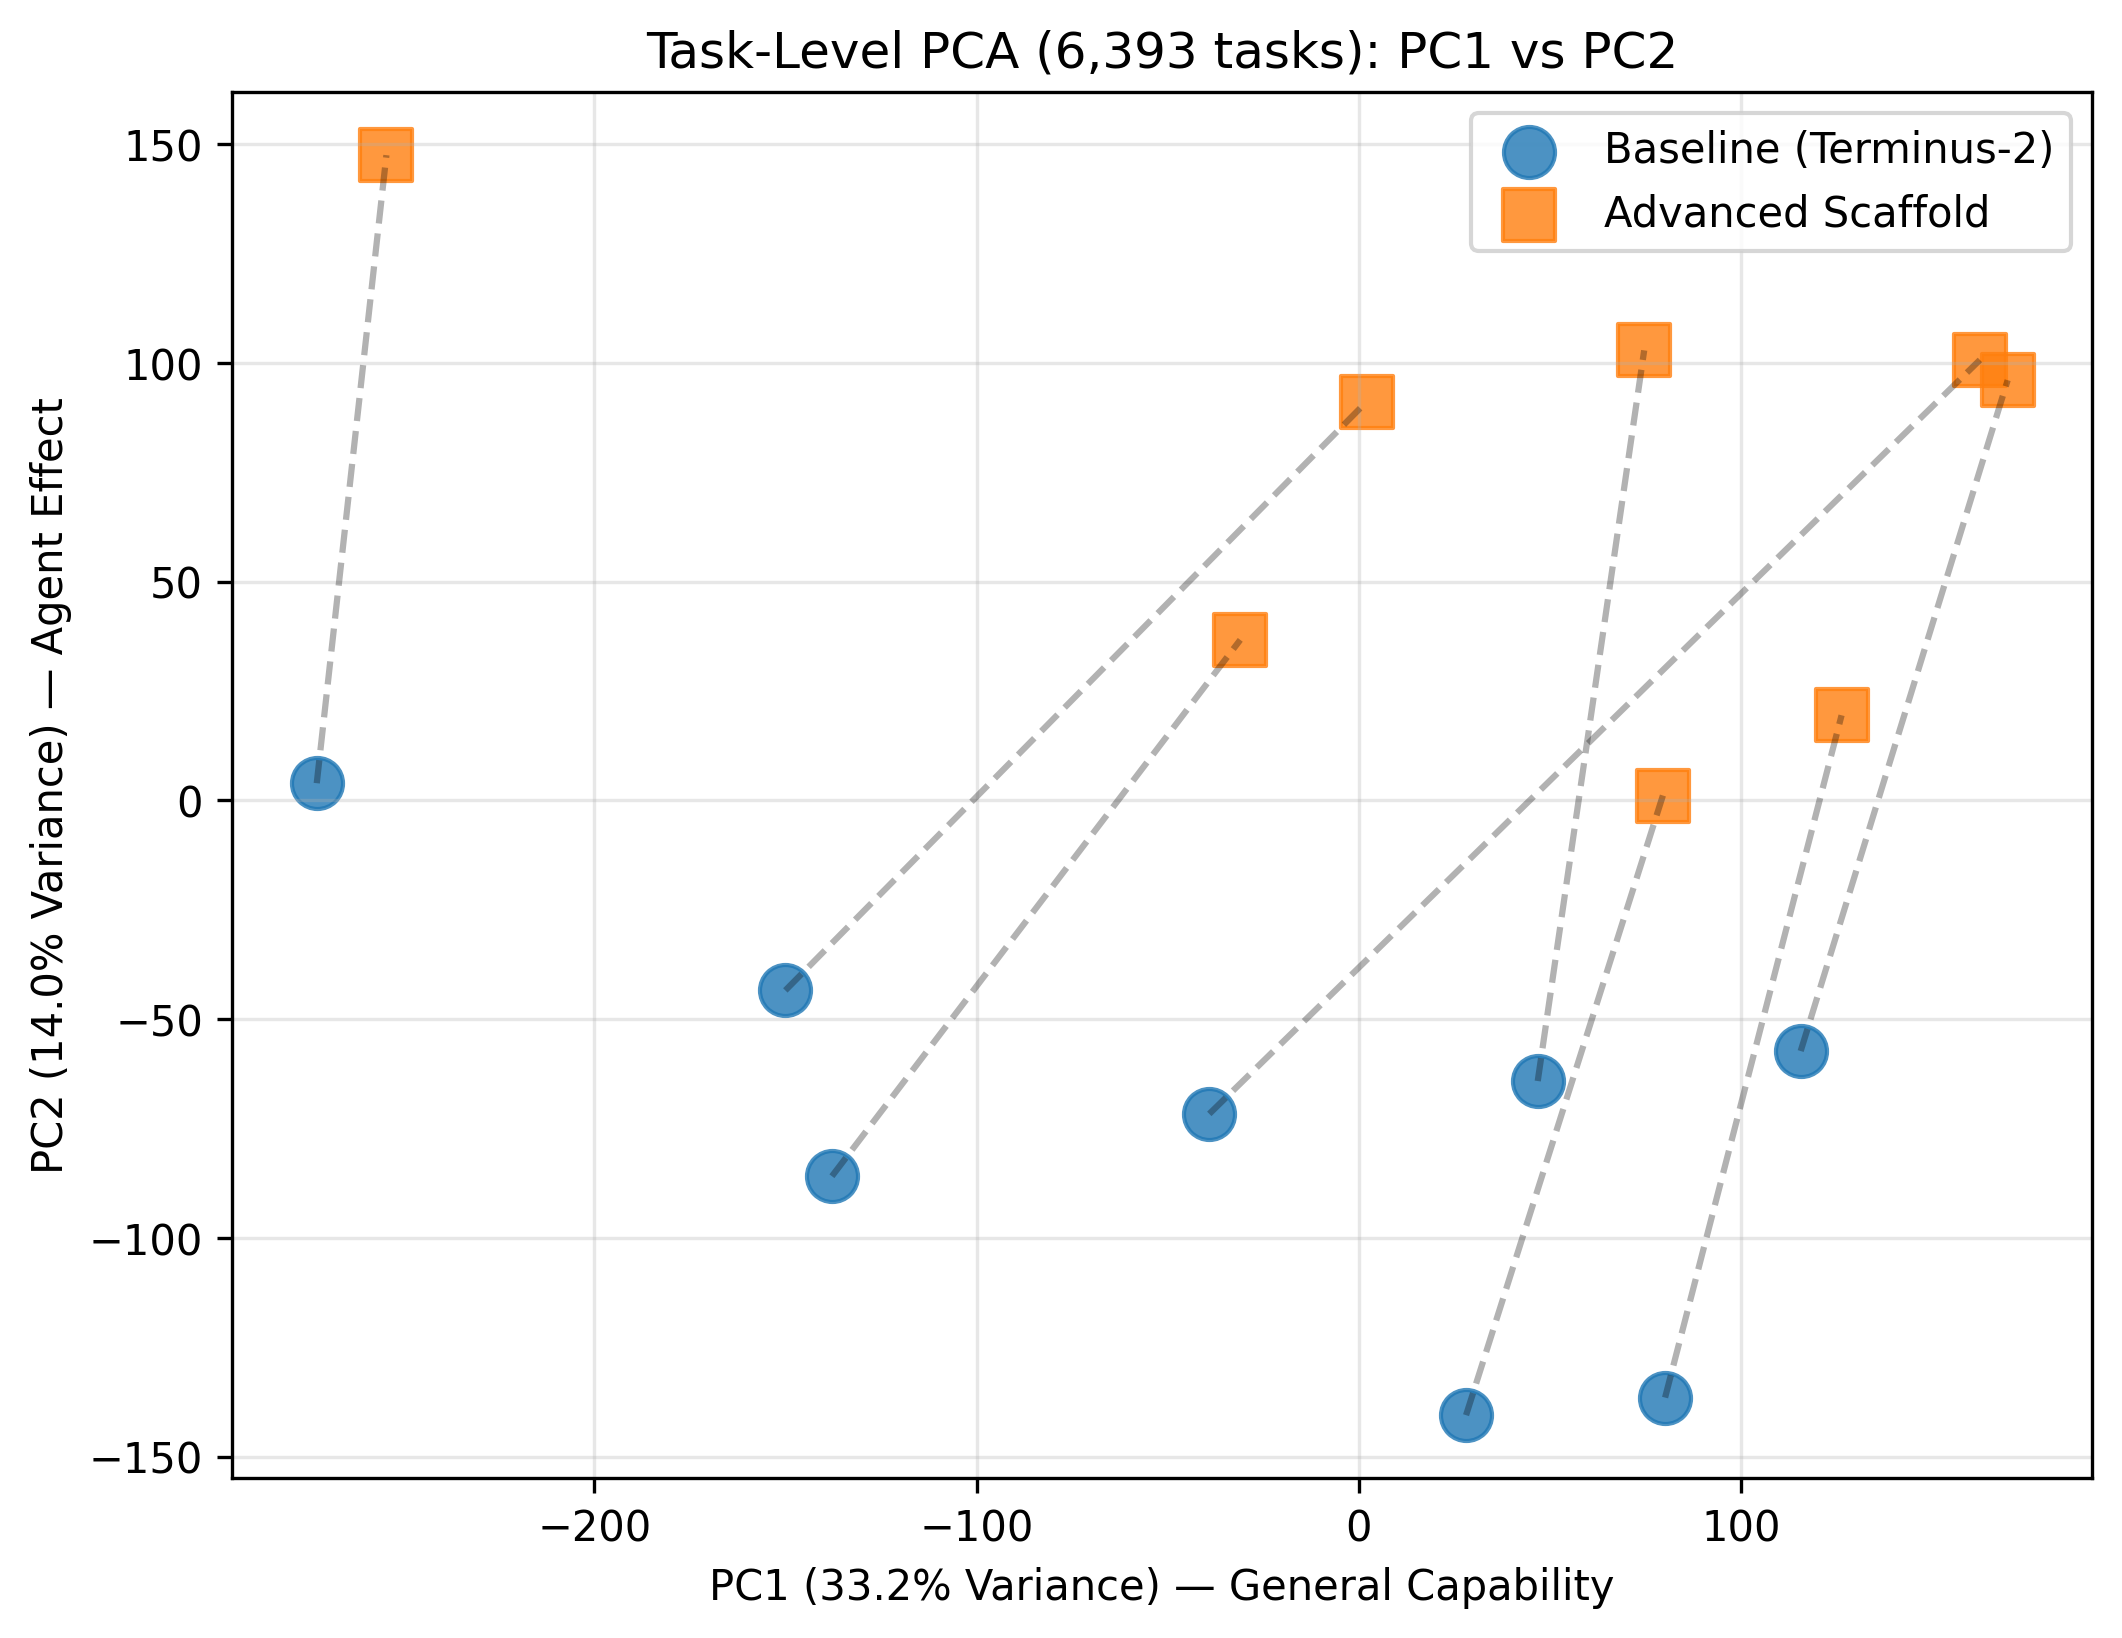
\includegraphics[width=0.7\linewidth]{figs/appendix/quantitative/task_level_pca.png}
%   \caption{Task-level PCA (\TaskGoodTasks{} tasks) in logit space. PC1 captures general capability, while PC2 perfectly isolates the effect of agent scaffolding. Dashed lines connect each baseline system to its advanced-scaffold counterpart.}
%   \label{fig:task-svd}
% \end{figure}

\paragraph{Limitations of Task-Level Prediction.}
Although the SVD spectrum is highly informative, applying the full BenchPress predictive pipeline (LogitBenchReg) to the task level fails due to the curse of dimensionality. With \TaskGoodTasks{} tasks and only $\AppNumSystems{}{-}1$ training systems (in a leave-one-out setup), finding the ``top 5 most correlated tasks'' guarantees a spurious training $R^2 = 1.000$ purely by chance, rendering out-of-sample predictions meaningless. Furthermore, task-level outcomes are predominantly binary (pass/fail), making continuous logit-OLS regression mathematically ill-suited. Therefore, for task-level redundancy and predictability, we rely on Item Response Theory principles (item-total correlation) rather than continuous matrix completion.

%%%%%%%%%%%%%%%%%%%%%%%%%%%%%%%%%%%%%%%%%%%%%%%%%%%%%%%%%%%%%%%%%%%%%%%%%%%%%%%

\subsubsection{Model vs.\ Agent Effect: Methodology Details}
\label{app:model-vs-agent}

This appendix formalizes the within-family and adjusted-effect analyses
summarized in Section~\ref{sec:agent-harness}.  Let $s(m, a, b)$ denote the
benchmark score for model~$m$, agent scaffold~$a$, and benchmark~$b$.

%%%%%%%%%%%%%%%%%%%%%%%%%%%%%%%%%%%%%%%%%%%%%%%%%%%%%%%%%%%%%%%%%%%%%%%%%%%%%%%
\paragraph{Within-Family Comparison}
\label{app:within-family}

For each model provider family $f$ (e.g., Anthropic, OpenAI, Google), let
$M_f$ be the set of models belonging to $f$ and $A_f$ the set of non-baseline
agents evaluated on that family.  The baseline agent is Terminus~2.

\subparagraph{Model effect (fixing agent).}
For each benchmark~$b$, we fix the agent to Terminus~2 and measure the score
range across models within the family:
\begin{equation}
  \Delta_{\mathrm{model}}^{(f,b)}
  \;=\;
  \max_{m \in M_f}\, s(m,\,\text{terminus-2},\,b)
  \;-\;
  \min_{m \in M_f}\, s(m,\,\text{terminus-2},\,b).
  \label{eq:model-effect}
\end{equation}
This requires at least two models in~$f$ with observed Terminus~2 scores on~$b$.

\subparagraph{Agent effect (fixing model).}
For each model $m \in M_f$ evaluated under both Terminus~2 and another agent
$a \in A_f$ on benchmark~$b$, we compute the absolute score change:
\begin{equation}
  \delta_{\mathrm{agent}}^{(m,a,b)}
  \;=\;
  \bigl|\, s(m,\,a,\,b) - s(m,\,\text{terminus-2},\,b) \,\bigr|.
  \label{eq:agent-delta}
\end{equation}
The family-level agent effect on~$b$ averages over all available model--agent pairs:
\begin{equation}
  \Delta_{\mathrm{agent}}^{(f,b)}
  \;=\;
  \frac{1}{|\mathcal{P}_{f,b}|}
  \sum_{(m,a)\in \mathcal{P}_{f,b}}
  \delta_{\mathrm{agent}}^{(m,a,b)},
  \label{eq:agent-effect}
\end{equation}
where $\mathcal{P}_{f,b} = \{(m,a) : m \in M_f,\; a \in A_f,\; \text{both }
s(m,a,b) \text{ and } s(m,\text{terminus-2},b) \text{ are observed}\}$.

\subparagraph{Dominance classification.}
For a given $(f, b)$ pair, the benchmark is classified as
\emph{model-dominant} if $\Delta_{\mathrm{model}}^{(f,b)} >
\Delta_{\mathrm{agent}}^{(f,b)}$, and \emph{agent-dominant} otherwise.

\subparagraph{Family-level summary.}
We aggregate across benchmarks within each family using the mean:
\begin{align}
  \overline{\Delta}_{\mathrm{model}}^{(f)}
  &= \frac{1}{|B_f|}\sum_{b \in B_f} \Delta_{\mathrm{model}}^{(f,b)}, &
  \overline{\Delta}_{\mathrm{agent}}^{(f)}
  &= \frac{1}{|B_f|}\sum_{b \in B_f} \Delta_{\mathrm{agent}}^{(f,b)},
  \label{eq:family-summary}
\end{align}
where $B_f$ is the set of benchmarks with both model-effect and agent-effect
estimates for family~$f$.  The model-to-agent ratio is
$\overline{\Delta}_{\mathrm{model}}^{(f)} / \overline{\Delta}_{\mathrm{agent}}^{(f)}$,
and the model-dominant percentage is the fraction of benchmarks in~$B_f$
classified as model-dominant.

Table~\ref{tab:within-family-summary} reports these statistics for the three
multi-model families.

\begin{table}[t]
  \centering
  \caption{Within-family model vs.\ agent effect comparison.  The model effect
    is the score range across models within the family on Terminus~2; the agent
    effect is the mean absolute score change from switching the agent while
    holding the model fixed.  Ratio and model-dominant percentage are computed
    per benchmark, then averaged.}
  \label{tab:within-family-summary}
  \begin{tabular}{lcccccc}
    \toprule
    Family
      & Models
      & Agents
      & $\overline{\Delta}_{\mathrm{model}}$
      & $\overline{\Delta}_{\mathrm{agent}}$
      & Ratio
      & Model-dom.\ \% \\
    \midrule
    Anthropic
      & 3
      & claude-code
      & \AnthropicModelEffectMean{}
      & \AnthropicAgentEffectMean{}
      & \AnthropicModelAgentRatio{}$\times$
      & \AnthropicModelWinPct\% \\
    OpenAI
      & 3
      & codex
      & \OpenAIModelEffectMean{}
      & \OpenAIAgentEffectMean{}
      & \OpenAIModelAgentRatio{}$\times$
      & \OpenAIModelWinPct\% \\
    Google
      & 2
      & gemini-cli
      & \GoogleModelEffectMean{}
      & \GoogleAgentEffectMean{}
      & \GoogleModelAgentRatio{}$\times$
      & \GoogleModelWinPct\% \\
    \bottomrule
  \end{tabular}
\end{table}

Table~\ref{tab:within-family-example} illustrates the per-benchmark comparison
for one representative family.

\begin{table}[t]
  \centering
  \caption{Example within-family comparison for the Anthropic family
    (claude-opus-4-6, claude-sonnet-4-6, claude-haiku-4-5).
    \emph{Model effect}: score range across the three models on Terminus~2.
    \emph{Agent effect}: mean $|\Delta|$ from switching to Claude~Code while
    holding each model fixed.  Only a representative subset of benchmarks is
    shown.}
  \label{tab:within-family-example}
  \small
  \begin{tabular}{lcccc}
    \toprule
    & \multicolumn{2}{c}{Model effect (Terminus-2)}
    & \multicolumn{2}{c}{Agent effect (fix model)} \\
    \cmidrule(lr){2-3}\cmidrule(lr){4-5}
    Benchmark & Score range & Rank & Mean $|\Delta|$ & Rank \\
    \midrule
    \multicolumn{5}{c}{\emph{Auto-populated from pipeline output ---
      see \texttt{benchmark\_within\_family\_model\_vs\_agent.csv}}} \\
    \bottomrule
  \end{tabular}
\end{table}


%%%%%%%%%%%%%%%%%%%%%%%%%%%%%%%%%%%%%%%%%%%%%%%%%%%%%%%%%%%%%%%%%%%%%%%%%%%%%%%
\subsubsection{Task-Level Redundancy Analysis}
\label{app:task-redundancy}
%%%%%%%%%%%%%%%%%%%%%%%%%%%%%%%%%%%%%%%%%%%%%%%%%%%%%%%%%%%%%%%%%%%%%%%%%%%%%%%

We extend the redundancy analysis from the benchmark level to the
individual task level.  Within each benchmark, we ask: how many tasks
are actually needed to reproduce the full benchmark ranking of
\AppNumSystems{} systems?

\paragraph{Intra-benchmark dimensionality.}
For each benchmark with $\ge 10$ tasks, we apply PCA to the
\AppNumSystems{}-system $\times$ $T$ task score matrix (after removing
zero-variance tasks).  On average, the first principal component alone
explains \textbf{\TaskRedundMeanPCOne{}\%} of the variance across tasks
within a benchmark, and a median of only
\textbf{\TaskRedundMedianPCsNinety{} components} suffices for 90\%
cumulative variance---a
\textbf{\TaskRedundMeanCompression{}$\times$} compression ratio.

Some benchmarks are particularly low-rank:
\begin{itemize}
  \item \textbf{\TaskLowRankExTwoName{}} (\TaskLowRankExTwoTasks{}
    tasks): PC1 = \TaskLowRankExTwoPCOne{}\%, only
    \TaskLowRankExTwoPCs{}~components for 90\%.
  \item \textbf{\TaskLowRankExThreeName{}} (\TaskLowRankExThreeTasks{}
    tasks): PC1 = \TaskLowRankExThreePCOne{}\%,
    \TaskLowRankExThreePCs{}~components for 90\%.
  \item \textbf{\TaskLowRankExOneName{}} (\TaskLowRankExOneTasks{}
    tasks): PC1 = \TaskLowRankExOnePCOne{}\%,
    \TaskLowRankExOnePCs{}~components for 90\%.
\end{itemize}
These benchmarks contain hundreds of items that essentially measure
the same underlying capability axis.

\paragraph{Representative task selection.}
We select the $k$ tasks with the highest Spearman correlation to the
full benchmark mean score, then measure how well the $k$-task subset
preserves the system ranking (Table~\ref{tab:task-redundancy}).

\begin{table}[t]
  \centering
  \caption{System ranking fidelity ($\rho$) from a small task subset
    vs.\ the full benchmark.  Values are mean Spearman rank
    correlation across all benchmarks with $\ge 10$ tasks.}
  \label{tab:task-redundancy}
  \begin{tabular}{cccc}
    \toprule
    $k$ tasks & Mean $\rho$ & Benchmarks $\rho > 0.95$ & Typical reduction \\
    \midrule
    1  & \TaskRedundRhoKOne{}  & \TaskRedundAboveNFKOne{}  & $>$100$\times$ \\
    3  & \TaskRedundRhoKThree{} & \TaskRedundAboveNFKThree{} & 30--60$\times$ \\
    5  & \TaskRedundRhoKFive{}  & \TaskRedundAboveNFKFive{}  & 20--40$\times$ \\
    10 & \TaskRedundRhoKTen{}   & \TaskRedundAboveNFKTen{}   & 10--20$\times$ \\
    \bottomrule
  \end{tabular}
\end{table}

With just 10 well-chosen tasks, \TaskRedundAboveNFKTen{} benchmarks
achieve $\rho > 0.95$---statistically indistinguishable from running
the full suite.  This complements the benchmark-level BenchPress finding
(Appendix~\ref{app:benchpress}): not only are many \emph{benchmarks}
redundant with each other, but within each benchmark most
\emph{tasks} are redundant as well.

\paragraph{Zero-variance tasks.}
An average of \TaskRedundMeanZeroVarPct{}\% of tasks per benchmark have
zero variance across all \AppNumSystems{} systems (all systems score 0
or all score 1).  These items provide no discriminative signal and can
be safely excluded.  Some benchmarks exhibit extreme saturation:
\texttt{\TaskZeroVarExOneName{}} (\TaskZeroVarExOnePct{}\%
zero-variance), \texttt{\TaskZeroVarExTwoName{}} (\TaskZeroVarExTwoPct{}\%),
\texttt{\TaskZeroVarExThreeName{}} (\TaskZeroVarExThreePct{}\%).

\paragraph{Implications.}
The two-level redundancy---across benchmarks
(Section~\ref{app:benchpress}) and within benchmarks (this
section)---implies that a carefully selected subset of benchmarks,
each evaluated on a small number of representative tasks, can
approximate the full evaluation matrix at a fraction of the
computational cost.  This motivates the HaborMix task selection
strategy described in the main text.
